\documentclass[UTF8]{ctexart}
\ctexset { section = { format={\Large \bfseries } } }
\pagestyle{plain}
\usepackage{float}
\usepackage{amsmath}
\usepackage{amssymb}
\usepackage{listings}
\usepackage{graphicx}
\usepackage{xcolor}
\usepackage{geometry}
\geometry{a4paper,scale=0.8}
\usepackage{caption}
\usepackage{subcaption}
\renewcommand{\abstractname}{\large Abstract}
\usepackage{booktabs}
\usepackage{siunitx}
\usepackage{multirow}
\usepackage[colorlinks=true, linkcolor=blue, citecolor=blue, urlcolor=blue]{hyperref}
\renewcommand{\refname}{References}
\captionsetup[figure]{name={Figure}}
\captionsetup[table]{name={Table}}
\definecolor{Rhodamine}{RGB}{227,11,92}

\lstset{
language=Python, % 设置语言
basicstyle=\ttfamily, % 设置字体族
breaklines=true, % 自动换行
keywordstyle=\bfseries\color{blue}, % 设置关键字为粗体,
morekeywords={}, % 设置更多的关键字,用逗号分隔
emph={self}, % 指定强调词,如果有多个,用逗号隔开
emphstyle=\bfseries\color{Rhodamine}, % 强调词样式设置
commentstyle=\color{black!50!white}, % 设置注释样式,斜体,浅灰色
stringstyle=\bfseries\color{red!90!black}, % 设置字符串样式
columns=flexible,
numbers=left, % 显示行号在左边
numbersep=2em, % 设置行号的具体位置
numberstyle=\footnotesize, % 缩小行号
frame=single, % 边框
framesep=1em % 设置代码与边框的距离
}

\title{\textbf{DATA130051.01 Computer Vision Midterm Project}}

\author{吴嘉骜 21307130203}
\date{June 2, 2024}

\setlength{\parindent}{0pt}

\begin{document}

\maketitle

\begin{abstract}
    \normalsize
    \noindent
    This report presents the completion of two tasks for the \textit{Computer Vision} Midterm Project.
    Task one involves fine-tuning a CNN pre-trained on ImageNet for bird species recognition. 
    We use ResNet-18 as the base network, pre-trained on ImageNet, and fine-tune the output layer on the CUB-200-2011 dataset. With a learning rate of 0.01 for the output layer and 0.001 for other parameters, 
    and training for 50 epochs, we achieve a test accuracy of 73.3\%.
    Task two involves training and testing object detection models Faster R-CNN and YOLO V3 on the VOC dataset. 
    We utilized MMDetection to train on the VOC2007 and VOC2012 train+val sets and tested on the VOC2007 test set. 
    Faster R-CNN achieves an mAP of 0.739, while YOLO V3 achieves an mAP of 0.420, each with 6 epochs of training.
    The report details the training specifics, performance metrics, and visualization results for both tasks.
\end{abstract}

\noindent
\textbf {Project description}\\  The objective of this project is to\\
1) fine-tune a pre-trained CNN on CUB-200-2011 for bird species recognition and \\
2) train and test object detection models Faster R-CNN and YOLO V3 on the VOC dataset.\\
The project aims to delve into the practical aspects of computer vision tasks.\\
\noindent
\textbf {Experiment environment} \\
    GPU: RTX 4090(24GB) * 1\\
    CPU: 16 vCPU Intel(R) Xeon(R) Gold 6430\\
    PyTorch  2.0.0  Python  3.8 (ubuntu20.04)  Cuda  11.8\\
    MMDetection 3.3.0\\
    More details can be found in the \texttt{requirements.txt} file in the project repository.\\
\noindent
\textbf {Model links} \\
Source code: \href{https://github.com/Julius-Woo/DATA130051.01-Computer-Vision/tree/main/Midterm}{Github link}\\
Model parameters: \href{https://pan.baidu.com/s/1O-toY96MSuXnaVT4yOSMvQ?pwd=92wa}{Baidu Netdisk link}\\


\section{Task 1: Fine-Tuning CNN}

\subsection{Introduction}
Image classification is a fundamental task in computer vision that involves categorizing images into predefined classes.
Fine-tuning is a transfer learning technique where a pre-trained neural network is adapted to a new but related task. 
This approach leverages the learned features of a large dataset, such as ImageNet, to improve performance on a smaller, domain-specific dataset.

In this task, we fine-tune a \textbf{ResNet-18 model}, pre-trained on ImageNet, for bird species recognition using the \textbf{CUB-200-2011} dataset. 
The goal is to achieve high accuracy in classification by tuning hyperparameters and demonstrate the effectiveness of transfer learning in contrast to training a model from scratch.

ResNet-18 is a convolutional neural network that uses residual learning to ease the training of deep networks. It consists of 18 layers, including convolutional layers, batch normalization layers, and identity shortcuts that skip one or more layers. These shortcuts mitigate the vanishing gradient problem and allow for the training of much deeper networks.

The architecture of ResNet-18 is as follows, shown in Figure \ref{fig:network}.
\begin{itemize}
    \item An initial convolutional layer with 64 filters and a 7x7 kernel, followed by a max-pooling layer.
    \item Four residual blocks, each containing two convolutional layers with 3x3 kernels.
    \item A global average pooling layer.
    \item A fully connected layer that outputs the final class scores.
\end{itemize}

\begin{figure}[H]
    \centering
    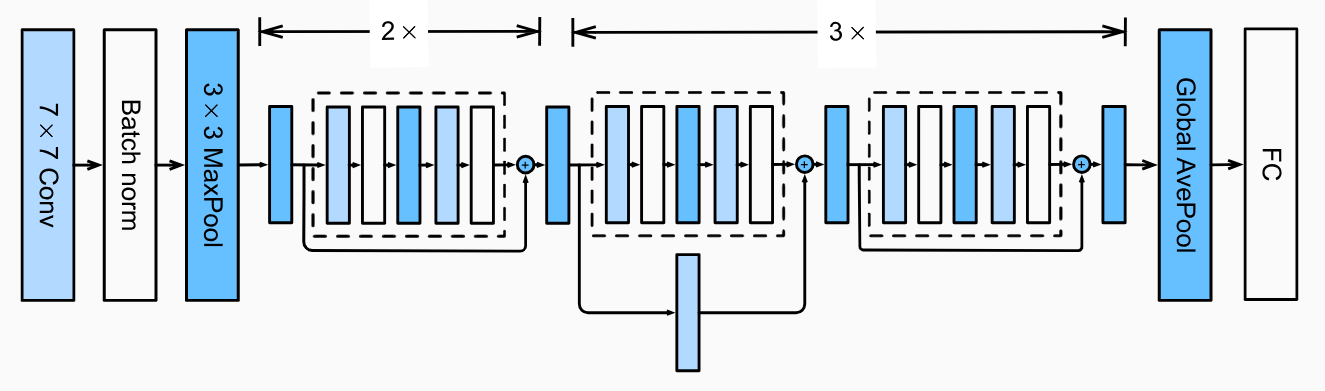
\includegraphics[width=0.7\textwidth]{./figs/resnet18.png}
    \caption{ResNet-18 Architecture}
    \label{fig:network}
\end{figure}

The \href{https://data.caltech.edu/records/65de6-vp158}{CUB-200-2011} dataset is a large-scale dataset for bird species recognition. It contains 11,788 images across 200 bird species, 5,994 for training and 5,794 for testing, 
with annotations for bounding boxes, part locations, and attributes. 
This dataset is commonly used for fine-grained image classification tasks due to its detailed annotations and variety of bird species.
In this task, we use the test set for evaluation and split the training set into 80\% for training and 20\% for validation randomly.

\subsection{Model Settings}
The model used for this task is a ResNet-18 model pre-trained on ImageNet, loaded from the PyTorch model zoo.
Its output layer is replaced with a new fully connected layer with 200 output units corresponding to the 200 bird species classes.
The model is then fine-tuned on the CUB-200-2011 dataset using the following hyperparameters:
\begin{itemize}
    \item Learning rate: 0.01 for the output layer and 0.001 for other parameters. Decay by a factor of 0.05 every 10 epochs.
    \item Batch size: 64.
    \item Number of epochs: 50.
    \item Loss function: Cross-entropy loss.
    \item Optimizer: Stochastic Gradient Descent (SGD) with momentum of 0.9.
    \item Regularization: L2 regularization with weight decay of 0.01.
    \item Data augmentation: Random resized cropping and horizontal flipping for training data.
    \item Early stopping: Stop training if validation loss does not improve for 5 epochs.
\end{itemize}


\subsection{Data Preprocessing and Augmentation}
For the CUB-200-2011 dataset, the following steps were performed:
\begin{itemize}
    \item \textbf{Training data:}
    \begin{itemize}
        \item Randomly resized cropping to 224x224 pixels.
        \item Random horizontal flipping.
        \item Conversion to tensor.
        \item Normalization with mean [0.485, 0.456, 0.406] and standard deviation [0.229, 0.224, 0.225].
    \end{itemize}
    \item \textbf{Validation and test data:}
    \begin{itemize}
        \item Resizing to 256x256 pixels.
        \item Center cropping to 224x224 pixels.
        \item Conversion to tensor.
        \item Normalization with mean [0.485, 0.456, 0.406] and standard deviation [0.229, 0.224, 0.225].
    \end{itemize}
\end{itemize}

\subsection{Hyperparameter Tuning}
To optimize the model's performance, hyperparameter tuning was conducted using grid search.

First, we tune the learning rates for the output layer and other parameters, with other hyperparameters fixed.
This is done by training the model for 15 epochs with weight decay 0.01, and evaluating the validation accuracy.
The result is shown in Table \ref{tab:lr}.

We find that a learning rate of 0.001 for other parameters and 0.01 for the output layer achieves the best validation accuracy of 71.06\%.

\begin{table}[h]
    \centering
    \caption{Learning Rate Results}
    \label{tab:lr}
    \begin{tabular}{|c|c|c|c|c|c|c|c|}
    \hline
    \textbf{LR o.w.} & \textbf{LR output} & \textbf{Train Acc} & \textbf{Val Acc} & \textbf{Test Acc} & \textbf{Best Val Acc} \\ \hline
    0.01 & 0.1 & 0.5078 & 0.4178 & 0.5074 & 0.4904 \\ \hline
    0.01 & 0.01 & 0.5969 & 0.4879 & 0.5690 & 0.5596 \\ \hline
    \textbf{0.001} & \textbf{0.01} & \textbf{0.7358} & \textbf{0.7048} & \textbf{0.7164} & \textbf{0.7106} \\ \hline
    0.001 & 0.001 & 0.5994 & 0.5997 & 0.6134 & 0.5997 \\ \hline
    0.0005 & 0.005 & 0.6970 & 0.6747 & 0.6964 & 0.6747 \\ \hline
    0.0001 & 0.001 & 0.4655 & 0.4762 & 0.4926 & 0.4762 \\ \hline
    1e-05 & 0.0001 & 0.0265 & 0.0242 & 0.0250 & 0.0250 \\ \hline
    5e-05 & 0.0005 & 0.2776 & 0.2702 & 0.2922 & 0.2702 \\ \hline
    \end{tabular}
\end{table}

Then, we find the best number of epochs for training with the optimal learning rates. This is under
the setting of above optimal learning rates, and weight decay 0.01.
The result is shown in Table \ref{tab:epochs}.

\begin{table}[h]
    \centering
    \caption{Epoch Results}
    \label{tab:epochs}
    \begin{tabular}{|c|c|c|c|c|}
    \hline
    \textbf{Epochs} & \textbf{Train Acc} & \textbf{Val Acc} & \textbf{Test Acc} & \textbf{Best Val Acc} \\ \hline
    15 & 0.7426 & 0.7056 & 0.7194 & 0.7056 \\ \hline
    25 & \textbf{0.8017} & 0.7248 & 0.7347 & 0.7248 \\ \hline
    45 & 0.8367 & 0.7206 & 0.7453 & 0.7381 \\ \hline
    65 & 0.8659 & \textbf{0.7323} & \textbf{0.7503} & \textbf{0.7456} \\ \hline
    \end{tabular}
    \end{table}
We find that generally, the model's performance improves with more epochs, but the validation accuracy plateaus after 25 epochs.
To prevent overfitting, we choose to train the model for around 50 epochs.

Finally, we search for the best weight decay value with the optimal learning rates.
The result is shown in Table \ref{tab:wd}. This is done by training the model for 25 epochs to save time.

\begin{table}[h]
    \centering
    \caption{Weight Decay Results}
    \label{tab:wd}
    \begin{tabular}{|c|c|c|c|c|}
    \hline
    \textbf{L2} & \textbf{Train Acc} & \textbf{Val Acc} & \textbf{Test Acc} & \textbf{Best Val Acc} \\ \hline
    0.1    & 0.1007 & 0.1243 & 0.3907 & 0.3770 \\ \hline
    0.01   & 0.7931 & 0.7189 & \textbf{0.7301} & \textbf{0.725} \\ \hline
    0.001  & 0.8482 & 0.7198 & 0.7275 & 0.7248 \\ \hline
    0.0001 & \textbf{0.8515} & \textbf{0.7198} & 0.7287 & 0.7206 \\ \hline
    \end{tabular}
    \end{table}

Although the model achieves the best training accuracy with the least weight decay 0.01,
it presents serious overfitting issues with the validation accuracy. 
We choose weight decay 0.01 to balance the trade-off between training and validation accuracy.

\subsection{Experiment Results}
We trained the ResNet-18 model on the CUB-200-2011 dataset with the optimal hyperparameters determined from the tuning process,
as listed in Model Settings. To prevent overfitting, we used early stopping with a patience of 5 epochs.
After 28 epochs, the patience is triggered, and the training is stopped early.
We achieve an accuracy of 77.23\% on the training set and 72.48\% on the validation set.
The test accuracy is 73.3\%.

The training and validation loss curves recorded in Tensorboard are shown in Figure \ref{fig:cubloss}.
\begin{figure}[h]
    \centering
    \begin{minipage}{0.45\textwidth}
        \centering
        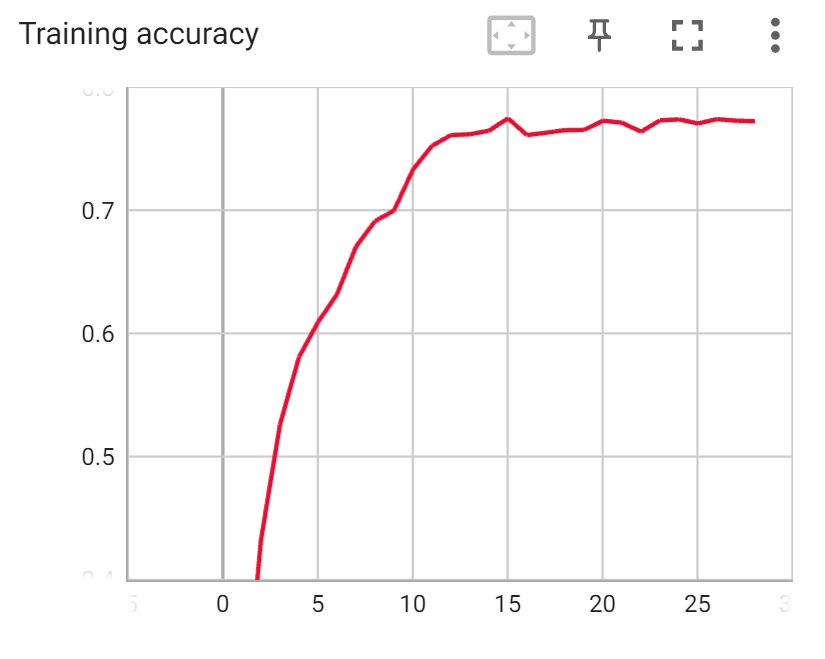
\includegraphics[width=\textwidth]{figs/TensorBoard/CUB_ft/ft_train_acc.png}
        \subcaption{Training Accuracy}
    \end{minipage}
    \hfill
    \begin{minipage}{0.45\textwidth}
        \centering
        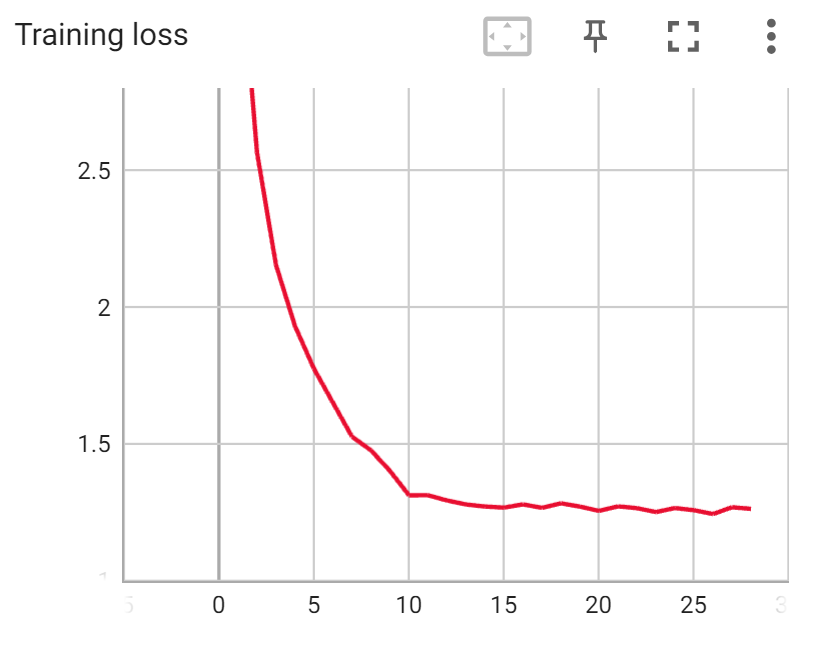
\includegraphics[width=\textwidth]{figs/TensorBoard/CUB_ft/ft_train_loss.png}
        \subcaption{Training Loss}
    \end{minipage}

    \vspace{0.5cm} % Adds some vertical space between rows

    \begin{minipage}{0.45\textwidth}
        \centering
        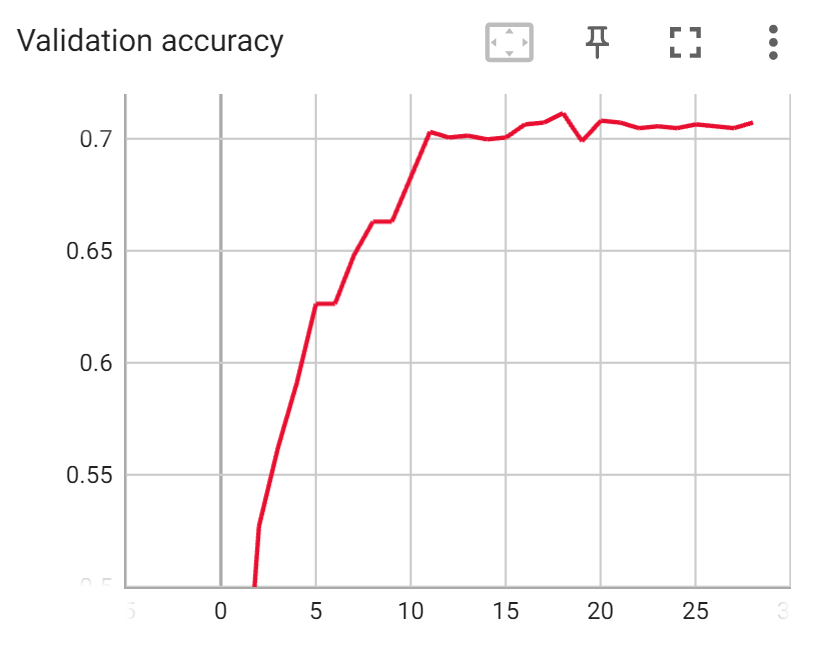
\includegraphics[width=\textwidth]{figs/TensorBoard/CUB_ft/ft_val_acc.png}
        \subcaption{Validation Accuracy}
    \end{minipage}
    \hfill
    \begin{minipage}{0.45\textwidth}
        \centering
        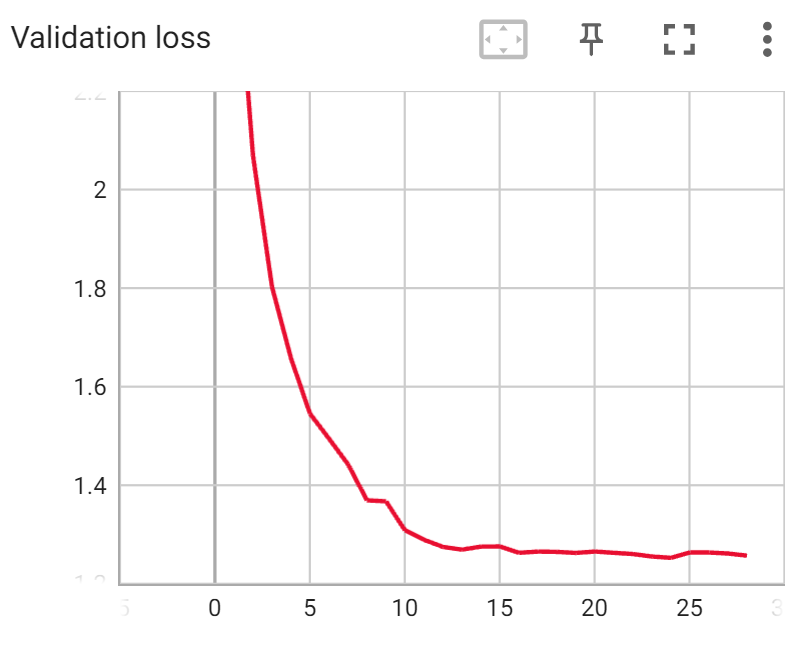
\includegraphics[width=\textwidth]{figs/TensorBoard/CUB_ft/ft_val_loss.png}
        \subcaption{Validation Loss}
    \end{minipage}
    \caption{Training and Validation Loss Curves for CUB-200-2011 Fine-Tuning}
    \label{fig:cubloss}
\end{figure}

\subsection{Discussion}
To demonstrate the effectiveness of transfer learning, we compare the results of fine-tuning a pre-trained ResNet-18 model
with training the same model from scratch on CUB-200-2011.
The latter model is initialized with random weights and trained with the same hyperparameters as the fine-tuned model, except that
the learning rate is set to 0.01 for all parameters to facilitate convergence and a longer training time of 100 epochs is used.
The TensorBoard loss curves for the scratch model are shown in Figure \ref{fig:scratchloss}.
The comparison results are shown in Table \ref{tab:comparison}.

\begin{table}[h]
    \centering
    \caption{Comparison of Pre-trained and Scratch ResNet-18 Models}
    \label{tab:comparison}
    \begin{tabular}{|l|c|c|}
    \hline
    \textbf{Metric} & \textbf{Pre-trained ResNet-18} & \textbf{Scratch ResNet-18} \\ \hline
    Training Epochs & 28 & 100 \\ \hline
    Train Acc & 0.7723 & 0.5447 \\ \hline
    Val Acc & 0.0.7248 & 0.3069 \\ \hline
    Test Loss & 1.1380 & 2.8258 \\ \hline
    Test Acc & \textbf{0.7325} & 0.3243 \\ \hline
    \end{tabular}
    \end{table}

    \begin{figure}[h]
        \centering
        \begin{minipage}{0.45\textwidth}
            \centering
            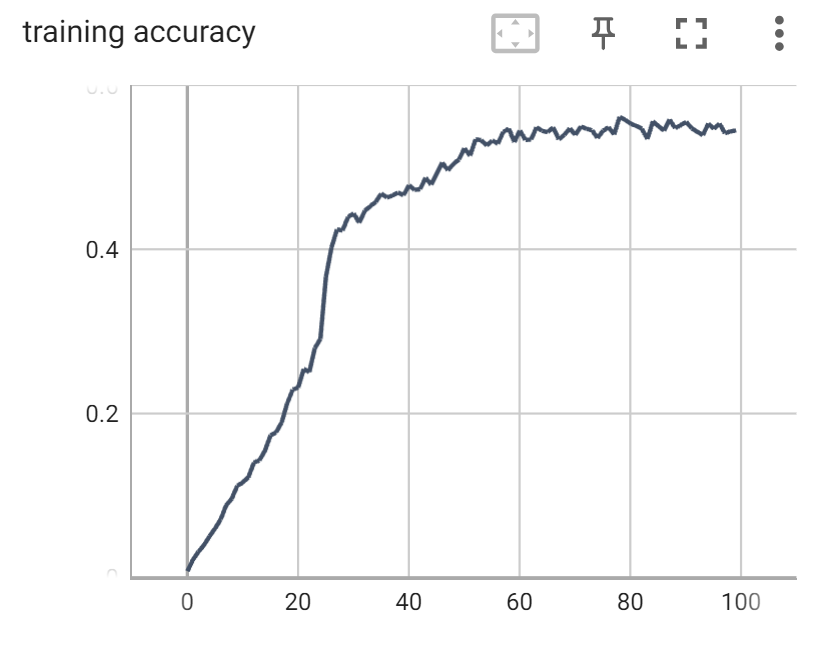
\includegraphics[width=\textwidth]{figs/TensorBoard/CUB_scratch/scratch_train_acc.jpg}
            \subcaption{Training Accuracy}
        \end{minipage}
        \hfill
        \begin{minipage}{0.45\textwidth}
            \centering
            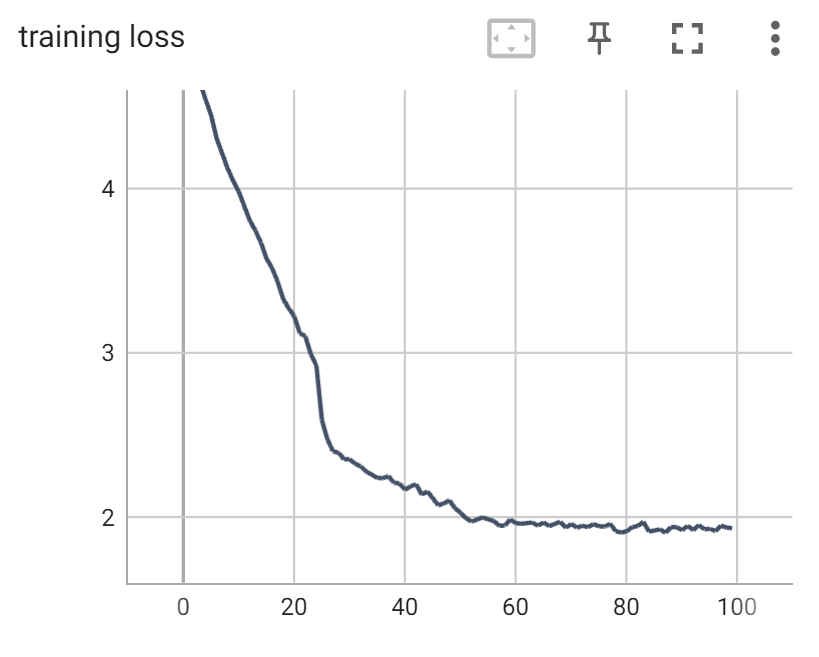
\includegraphics[width=\textwidth]{figs/TensorBoard/CUB_scratch/scratch_train_loss.jpg}
            \subcaption{Training Loss}
        \end{minipage}
    
        \vspace{0.5cm} % Adds some vertical space between rows
    
        \begin{minipage}{0.45\textwidth}
            \centering
            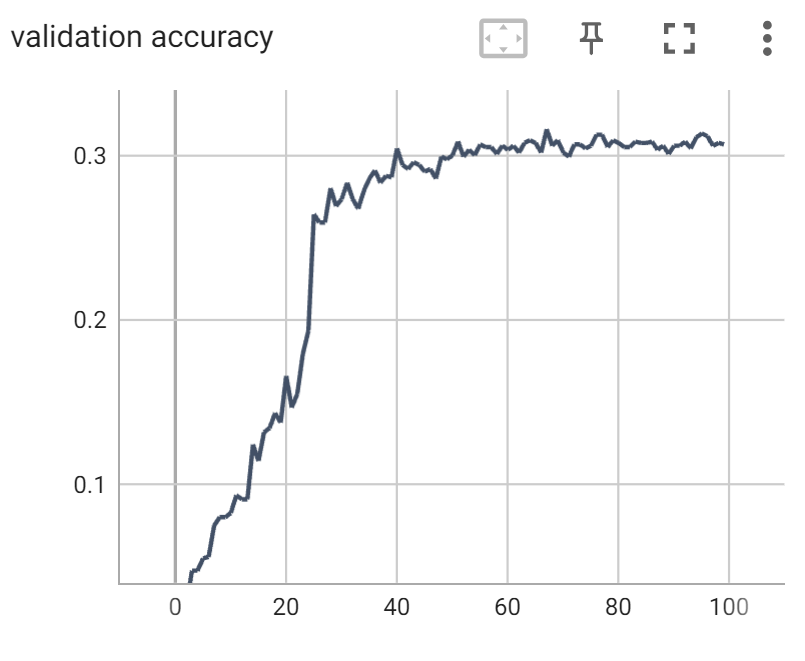
\includegraphics[width=\textwidth]{figs/TensorBoard/CUB_scratch/scratch_val_acc.png}
            \subcaption{Validation Accuracy}
        \end{minipage}
        \hfill
        \begin{minipage}{0.45\textwidth}
            \centering
            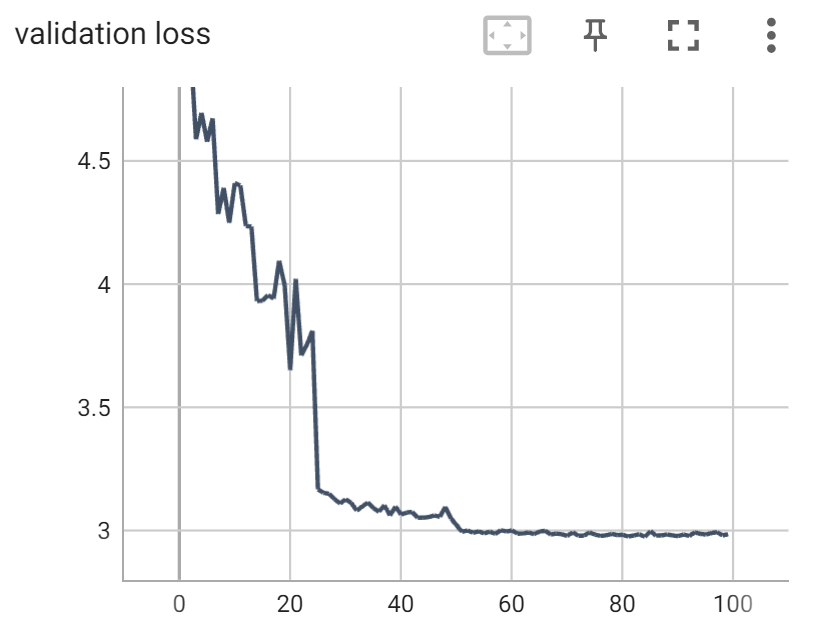
\includegraphics[width=\textwidth]{figs/TensorBoard/CUB_scratch/scratch_val_loss.png}
            \subcaption{Validation Loss}
        \end{minipage}
        \caption{Training and Validation Loss Curves for CUB-200-2011 Scratch Training}
        \label{fig:scratchloss}
    \end{figure}

This comparison demonstrates that the pre-trained ResNet-18 model significantly outperforms the scratch model, with much
fewer training epochs. This highlights the benefits of transfer learning in leveraging pre-trained models to improve performance on domain-specific tasks.

    
\section{Task 2: Object Detection}
\subsection{Introduction}
Object detection is a crucial task in computer vision that involves identifying and localizing objects within an image.
Unlike image classification, which only predicts the category of the entire image, 
object detection provides both the classes and bounding boxes of all objects present in the image.

In this task, we utilize two popular object detection models: \textbf{Faster R-CNN} and \textbf{YOLO V3} to perform object detection on the \textbf{PASCAL VOC} dataset.
The models are provided by the \textbf{MMDetection} framework, and we train them on the VOC2007 and VOC2012 train+val sets and evaluate them on the VOC2007 test set.
The goal is to compare the performance of these two models and analyze their generalization capabilities.

\begin{itemize}
    \item \textbf{Faster R-CNN:} Faster Region-based Convolutional Neural Network (Faster R-CNN) is a two-stage object detection model that first proposes candidate object regions and then classifies these regions into different object categories. The model consists of a Region Proposal Network (RPN) that generates region proposals and a Fast R-CNN detector that classifies the proposals and refines their bounding boxes. Its architecture is shown in Figure \ref{fig:faster_rcnn}.
    \item \textbf{YOLO V3:} You Only Look Once (YOLO) V3 is a single-stage object detection model that divides the image into a grid and directly predicts bounding boxes and class probabilities for each grid cell. YOLO V3 is known for its speed and efficiency, making it suitable for real-time applications. Its architecture is shown in Figure \ref{fig:yolo}.
\end{itemize}

\href{https://github.com/open-mmlab/mmdetection}{MMDetection} is an open-source object detection toolbox based on PyTorch. 
It provides a comprehensive framework for training and testing various object detection models, including Faster R-CNN and YOLO V3. MMDetection is designed to be flexible and extensible, allowing researchers to implement and evaluate new models with ease. It also includes a wide range of pre-trained models and utilities for data processing, model evaluation, and visualization.

For this task, we use the \href{http://host.robots.ox.ac.uk/pascal/VOC/}{PASCAL VOC} dataset, which is a standard benchmark for object detection. 
The dataset includes annotated images with objects from 20 categories such as animals, vehicles, and household items. Each image is annotated with bounding boxes and class labels.
We use the train+val sets from VOC2007 and VOC2012, totaling 16,551 images for training, and the test set from VOC2007, containing 4,952 images for evaluation.
This dataset's diversity and complexity make it ideal for evaluating object detection models.

\begin{figure}[H]
    \centering
    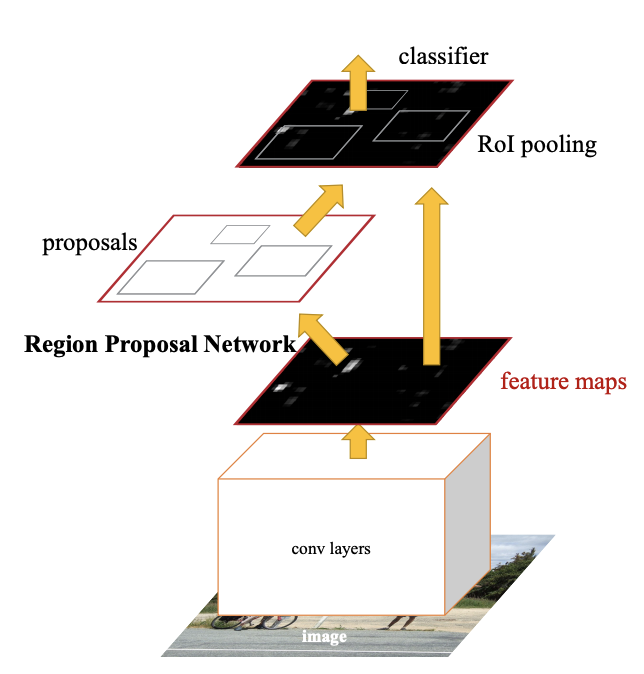
\includegraphics[width=0.45\textwidth]{./figs/faster-rcnn.png}
    \caption{Faster R-CNN Architecture}
    \label{fig:faster_rcnn}
\end{figure}

\begin{figure}[H]
    \centering
    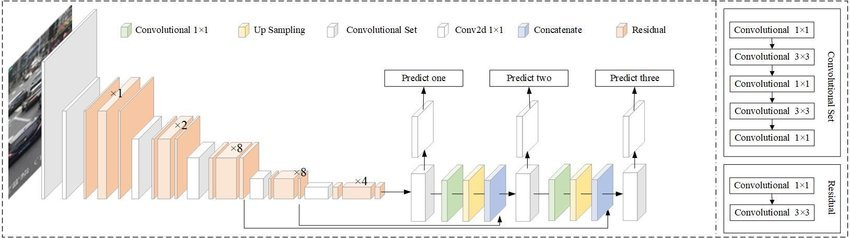
\includegraphics[width=0.5\textwidth]{./figs/YOLOv3.jpg}
    \caption{YOLO V3 Architecture}
    \label{fig:yolo}
\end{figure}

\subsection{Model Settings}
For our object detection experiments, we utilize the following configurations for the Faster R-CNN and YOLO V3 models.
Most configurations are based on the default settings provided by MMDetection such as IoU thresholds, NMS thresholds, and anchor ratios, with minor adjustments for the specific task.

\subsubsection{Faster R-CNN}
\begin{itemize}
    \item \textbf{Batch Size:} 2
    \item \textbf{Learning Rate:} The learning rate schedule follows a MultiStepLR policy, starting at 0.005 with milestones at epochs 2, 4, and 5, and a decay factor (gamma) of 0.05.
    \item \textbf{Optimizer:} SGD with a learning rate of 0.005, momentum of 0.9, and weight decay of 0.0001.
    \item \textbf{Iterations per Epoch:} 2476
    \item \textbf{Epochs:} 6
    \item \textbf{Loss Function:} The overall loss includes RPN classification loss, RPN bounding box regression loss, classification loss, and bounding box regression loss.
    \item \textbf{Evaluation Metric:} Mean Average Precision (mAP) for object detection performance.
\end{itemize}

\subsubsection{YOLO V3}
\begin{itemize}
    \item \textbf{Batch Size:} 2
    \item \textbf{Learning Rate:} The schedule starts with a LinearLR policy with a start factor of 5e-4, transitioning to a MultiStepLR policy with milestones at epochs 2, 4, and 5, and gamma of 0.1.
    \item \textbf{Optimizer:} SGD with a learning rate of 0.0001, momentum of 0.9, weight decay of 0.0005, and gradient clipping with a max norm of 35 and norm type of 2.
    \item \textbf{Iterations per Epoch:} 2476
    \item \textbf{Epochs:} 6
    \item \textbf{Loss Function:} The total loss includes classification loss, confidence loss, coordinate loss for x and y, and width/height loss.
    \item \textbf{Evaluation Metric:} mAP for object detection performance.
\end{itemize}

\subsection{Experiment Results}
We train the Faster R-CNN and YOLO V3 models on the VOC2007 and VOC2012 train+val sets as described in the Model Settings section.
After training for 6 epochs respectively, we achieve an mAP of 0.739 for Faster R-CNN and 0.420 for YOLO V3 on the validation set.

TensorBoard curves for Faster R-CNN and YOLO V3 are shown in Figure \ref{fig:fasterloss} and Figure \ref{fig:yololoss} respectively.

\begin{figure}[H]
    \centering
    \begin{minipage}{0.45\textwidth}
        \centering
        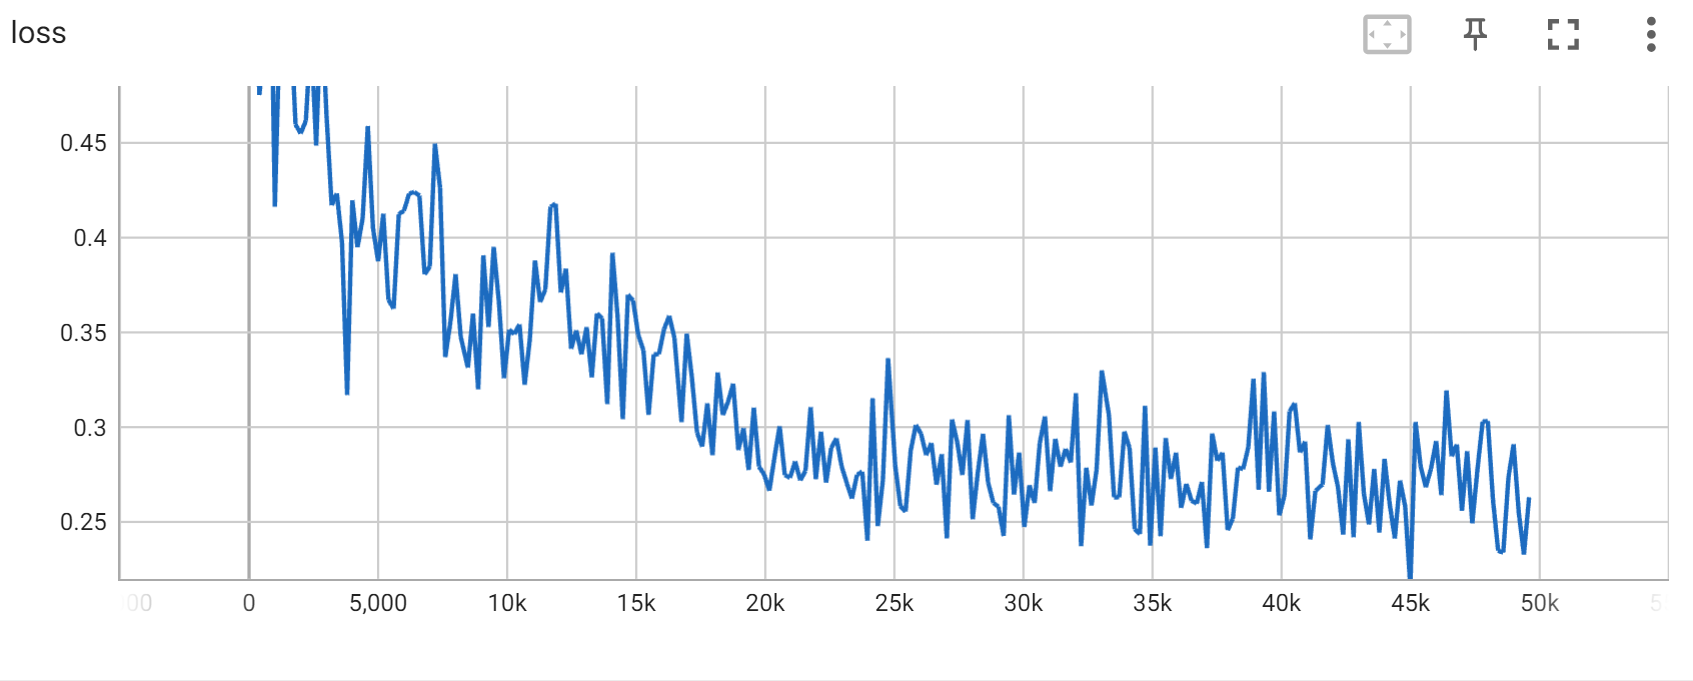
\includegraphics[width=\textwidth]{figs/TensorBoard/VOC_faster-rcnn/faster-rcnn_loss.png}
        \subcaption{Faster R-CNN Training Loss}
    \end{minipage}
    \hfill
    \begin{minipage}{0.45\textwidth}
        \centering
        \includegraphics[width=\textwidth]{figs/TensorBoard/VOC_faster-rcnn/faster-rcnn_mAP.png}
        \subcaption{Faster R-CNN mAP}
    \end{minipage}
    \caption{Training Loss and mAP Curves for Faster R-CNN}
    \label{fig:fasterloss}
\end{figure}

\begin{figure}[H]
    \centering
    \begin{minipage}{0.45\textwidth}
        \centering
        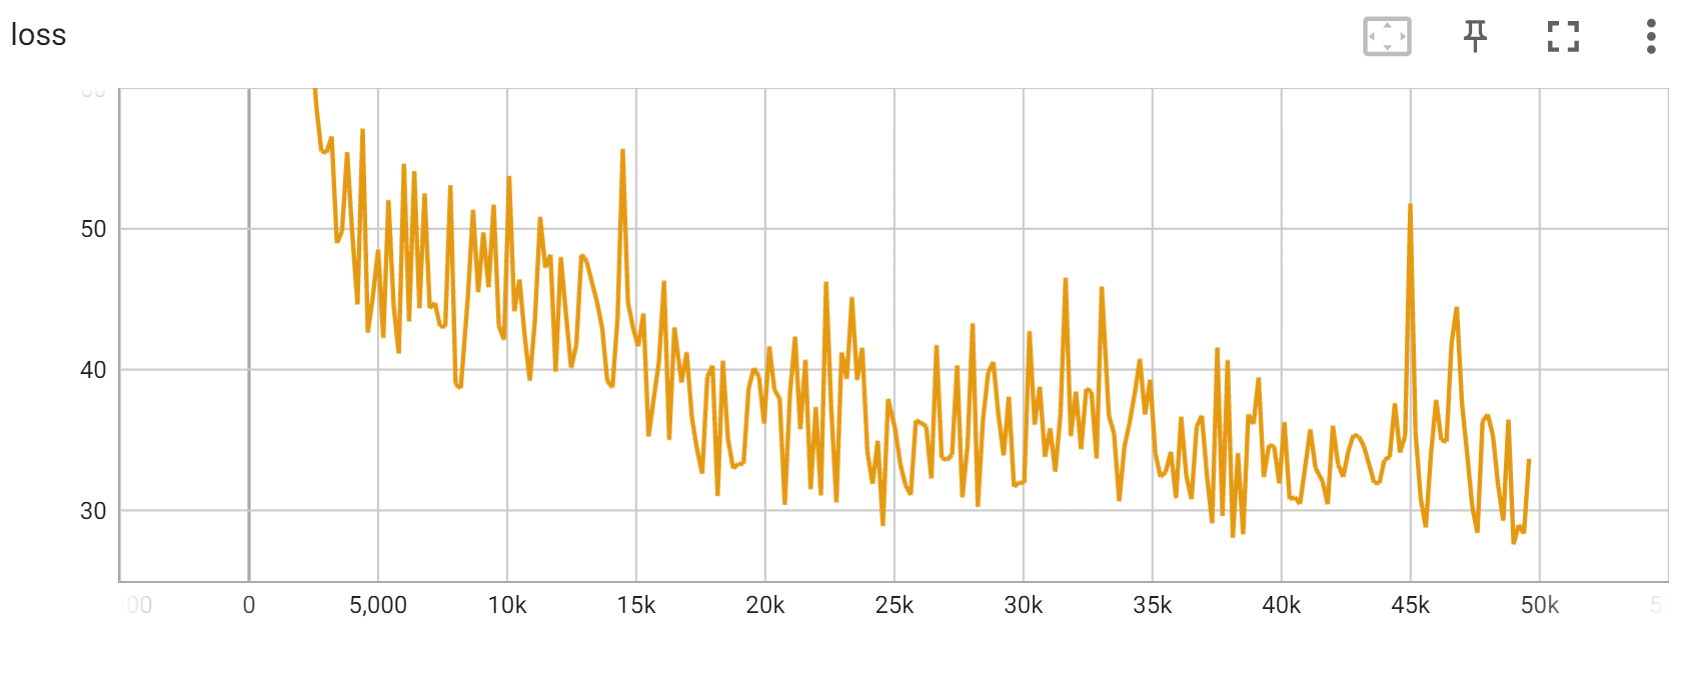
\includegraphics[width=\textwidth]{figs/TensorBoard/VOC_yolov3/yolo_loss.png}
        \subcaption{YOLO V3 Training Loss}
    \end{minipage}
    \hfill
    \begin{minipage}{0.45\textwidth}
        \centering
        \includegraphics[width=\textwidth]{figs/TensorBoard/VOC_yolov3/yolo_mAP.png}
        \subcaption{YOLO V3 mAP}
    \end{minipage}
    \caption{Training Loss and mAP Curves for YOLO V3}
    \label{fig:yololoss}
\end{figure}

\subsection{Faster R-CNN Visualization}
To illustrate the effectiveness of the two-stage object detection approach used in Faster R-CNN, 
we select four images from the test set. 
We compare the proposal boxes generated in the first stage with the final prediction results after the second stage, shown in Figure \ref{fig:faster_vis}.
We can see that the second stage refines the initial proposals, resulting in more accurate and reliable object detections.

The proposal boxes generated in the first stage provide a rough estimate of object locations, but they often include false positives and imprecise boundaries. The second stage refines these proposals, resulting in more accurate and reliable final predictions. This refinement process reduces false positives, improves localization accuracy, and enhances overall detection performance.
Thus, the second stage of Faster R-CNN plays a crucial role in improving the quality of object detection results.

\begin{figure}[H]
    \centering
    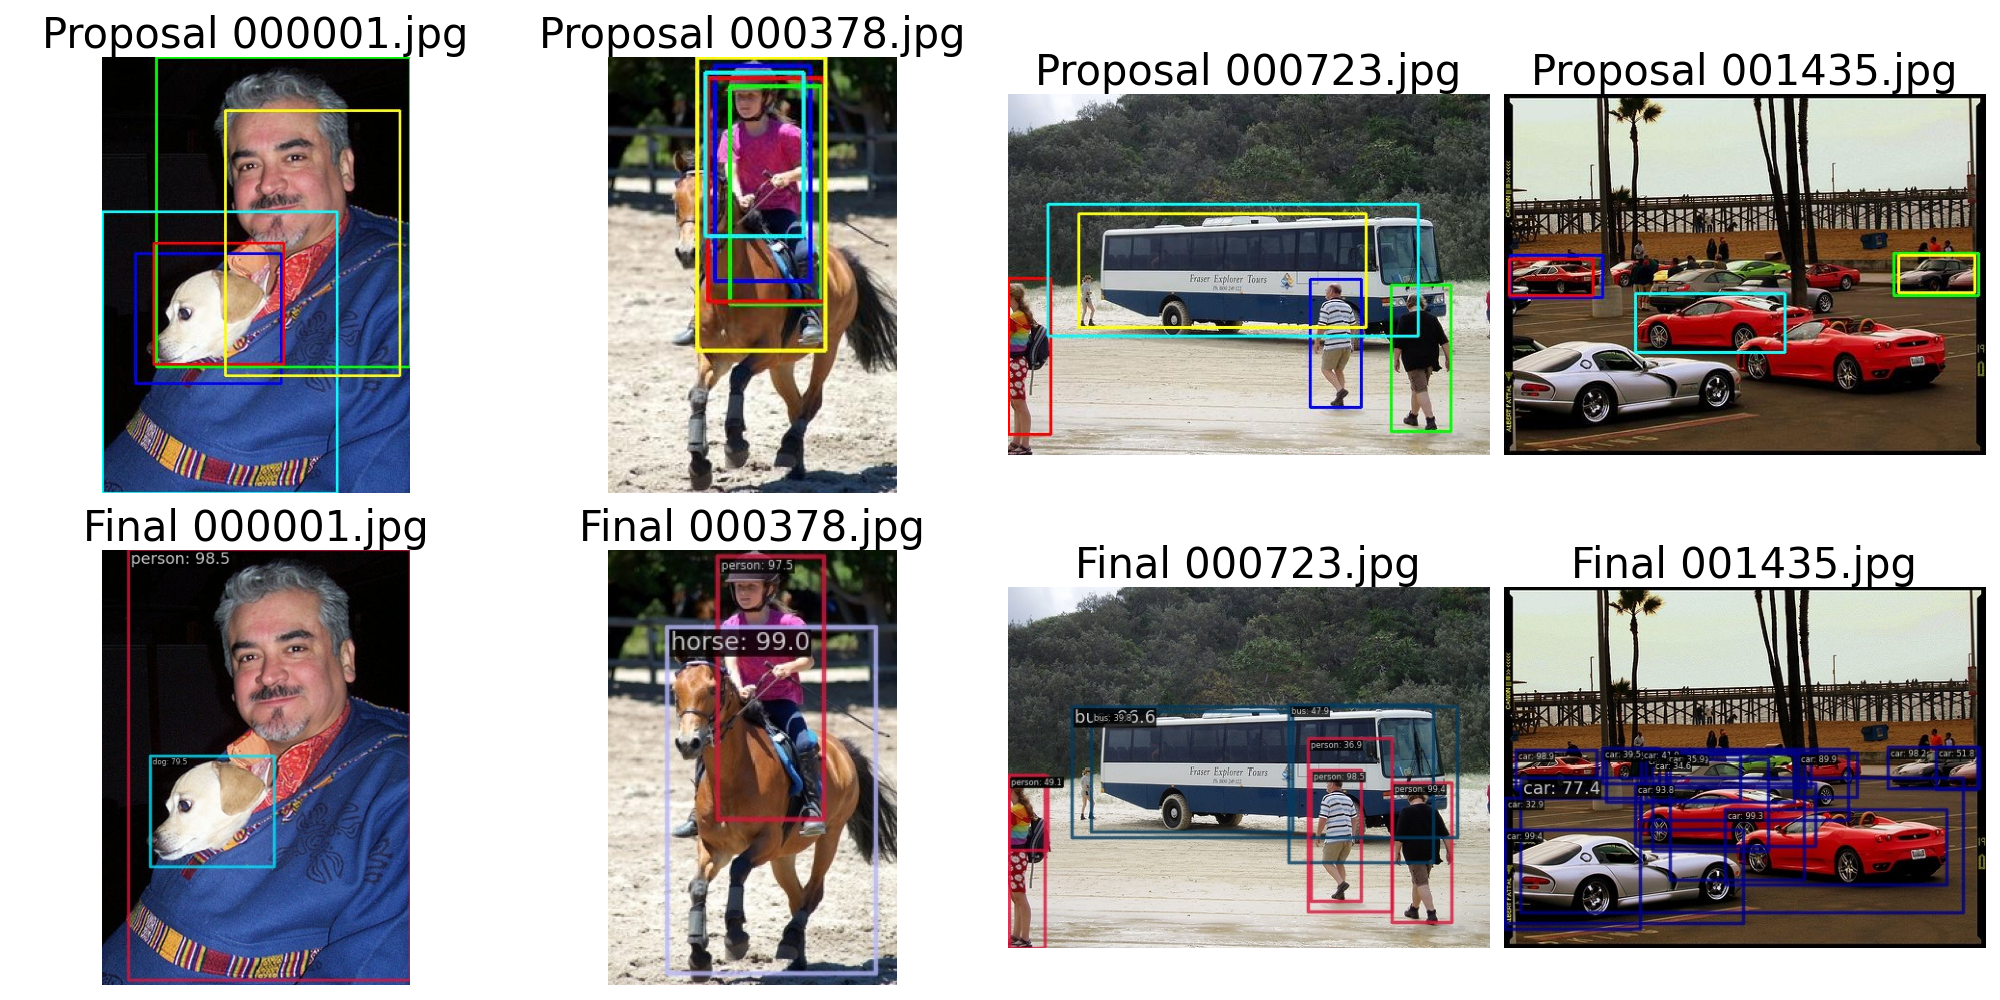
\includegraphics[width=1.0\textwidth]{./figs/faster-rcnn/comparison.png}
    \caption{Faster R-CNN Visualization}
    \label{fig:faster_vis}
\end{figure}


\subsection{Discussion}
To evaluate the generalization ability of the trained models, we collect three images that are not part of PASCAL VOC but contain objects from the VOC categories. 
We visualize and compare the detection results of the two models on these three images. 
Each image displays the bounding boxes, class labels, and confidence scores for the detected objects.
The visualization results are shown in Figure \ref{fig:external_vis}.

\begin{figure}[H]
    \centering
    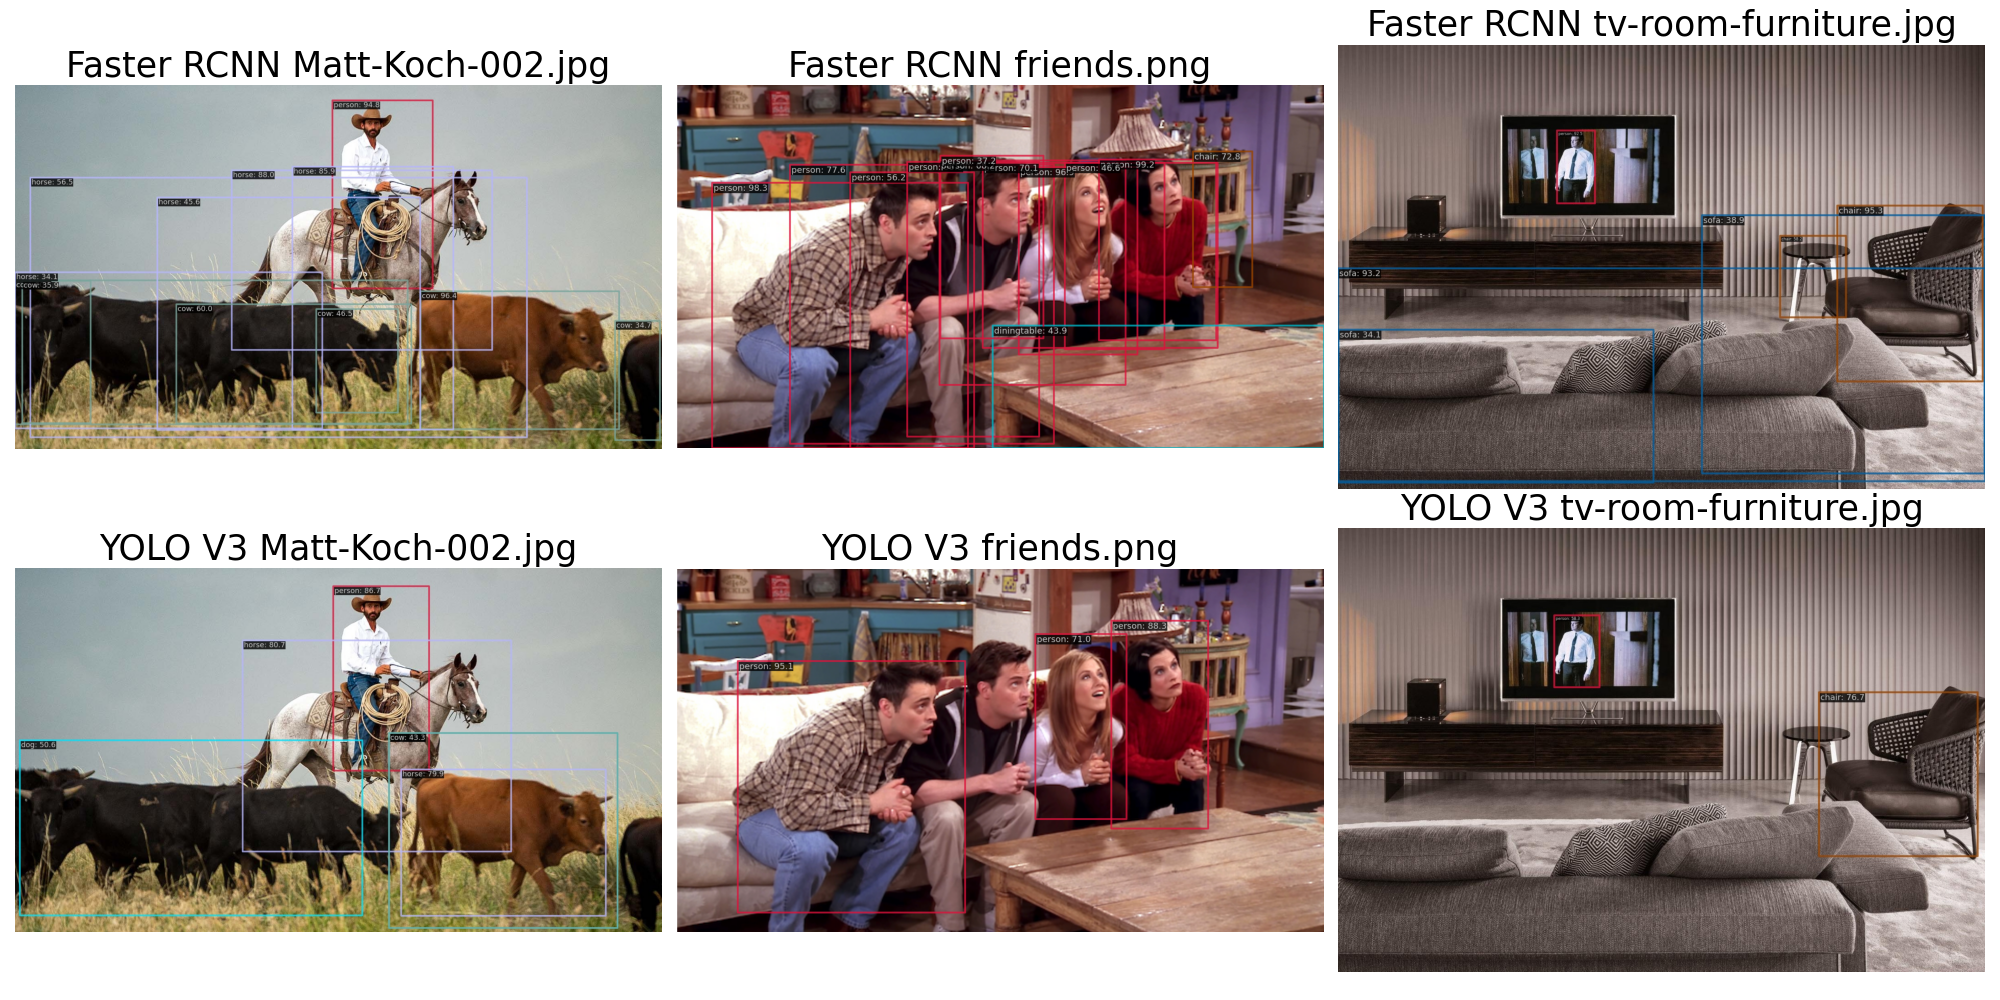
\includegraphics[width=1.0\textwidth]{./figs/external_comparison.png}
    \caption{Faster R-CNN Visualization}
    \label{fig:external_vis}
\end{figure}

We observe that Faster R-CNN predicts more accurate bounding boxes and class labels compared to YOLO V3, especially for images with numerous objects and occlusions.
For example, in the third image, Faster R-CNN successfully detects the sofa and table, while YOLO V3 fails to distinguish them. However, they both fail to detect the TV and only detect the person in the background.

Together with the training and validation results, as shown in Table \ref{tab:objcomparison}, we can see that Faster R-CNN outperforms YOLO V3 in many ways,
although it requires more training time. 
One possible reason for this could be that the number of training epochs was relatively low (to save time), 
which might have led to under-training of the YOLO V3 model. 
YOLO V3 typically benefits from longer training times to fully optimize its detection capabilities, 
whereas Faster R-CNN can achieve good performance with fewer epochs due to its two-stage detection process.

\begin{table}[h]
    \centering
    \caption{Comparison for Object Detection Models}
    \label{tab:objcomparison}
    \begin{tabular}{|c|c|c|c|}
    \hline
    \textbf{Model} & \textbf{Training Time} & \textbf{Epochs} & \textbf{mAP} \\ \hline
    Faster R-CNN & 74m 7.5s & 6 & 0.739 \\ \hline
    YOLO V3 & 61m 6.1s & 6 & 0.420 \\ \hline
    \end{tabular}
\end{table}

\section{Limitations and future work}
While the experiments yielded valuable insights, several limitations and potential areas for improvement were identified:

\begin{enumerate}
    \item \textbf{Limited Training Time and Hardware Constraints:} The accuracy and mAP scores of the trained models were not particularly high, likely due to the limited training time and hardware constraints. Allocating more time for training, utilizing more powerful hardware or utilizing more expressive models like ResNet-50
    could improve the performance.
    
    \item \textbf{Overfitting:} The current models showed signs of overfitting, as indicated by the gap between training and validation accuracy. This issue could be mitigated by incorporating regularization techniques such as Dropout layers to prevent overfitting.
    
    \item \textbf{Data Augmentation:} Implementing more sophisticated data augmentation techniques could help improve the models' generalization capabilities, especially for object detection tasks where robustness to variations in object appearance is crucial.
\end{enumerate}

\begin{thebibliography}{9}
\bibitem{}
Matt-Koch-002.jpg comes from \href{https://westernhorseman.com/culture/road-stories/matt-koch-is-simply-cowboy/}{Western Horseman}.
\bibitem{}
friends.png comes from the famous TV series \textit{Friends}.
\bibitem{}
tv-room-furniture.jpg comes from \href{https://minottilondon.com/set-up-tv-room/}{Minotti London}.
\bibitem{}
https://mmdetection.readthedocs.io/en/latest/
\end{thebibliography}

\end{document}